%\documentclass[aps,onecolumn,preprintnumbers,amsmath,amssymb,nofootinbib,superscriptaddress,notitlepage]{revtex4-1}
%\documentclass[preprint,12pt]{elsarticle}
\documentclass[5p,times]{elsarticle}
%\documentclass[aps,nofootinbib,prl,showpacs,twocolumn,groupedaddress,superscriptaddress]{revtex4}


\usepackage{graphicx}
\usepackage{dashrule}
\usepackage{dcolumn}
\usepackage{mathtools}
\usepackage{amssymb}
\usepackage{bbold}
\usepackage{amsmath}
\usepackage{amsfonts}
\usepackage{wasysym}
\usepackage{slashed}
\usepackage[dvipsnames]{xcolor}
\usepackage{soul}
\usepackage{rotating}
\usepackage{paracol}
\usepackage{nicefrac}
\usepackage{MnSymbol}

%\usepackage{subcaption}
%\newbox{\bigpicturebox}

\newcommand{\reales}{{\rm R}\hspace{-1ex}\rule{0.1mm}{1.5ex}\hspace{1ex}}
\def\tstrut{\vrule height2.5ex depth0pt width0pt} % used in tables
\def\jtstrut{\vrule height5ex depth0pt width0pt} % used in tables

\newcommand{\figref}[1]{fig.~(\ref{#1})}
\newcommand{\tabref}[1]{table~(\ref{#1})}
\newcommand{\ccite}[1]{ref.~\cite{#1}}

\newcommand{\eref}[1]{eq.~(\ref{#1})}
\newcommand{\eg}{\textit{e.g.}~}
\newcommand{\ie}{\textit{i.e.}~}
\newcommand{\viz}{\textit{viz.}~}
\newcommand{\cf}{\textit{cf.}~}
\newcommand{\eftnopi}{\mbox{EFT($\slashed{\pi}$) }}
\newcommand{\ve}[1]{\ensuremath{\boldsymbol{#1}}}
\newcommand{\rcm}{\ensuremath{\ve{R}_\text{\scriptsize{c.m.}}}}
\newcommand*{\mprime}{^{\prime}\mkern-1.2mu}
\newcommand*{\mdprime}{^{\prime\prime}\mkern-1.2mu}
\newcommand*{\mtprime}{^{\prime\prime\prime}\mkern-1.2mu}
\newcommand{\ddrei}[1]{\delta_{\tiny \lambda}^{(3)}\!\big(#1\big)}
\newcommand{\cc}{\ensuremath C(\lambda)}
\newcommand{\dd}{\ensuremath D(\lambda)}
\newcommand{\hbstwom}{\ensuremath \frac{\hbar^2}{2\mu}}
\newcommand{\twomhbs}{\ensuremath \frac{2\mu}{\hbar^2}}
\newcommand{\coup}[3]{\left[\,#1\,\otimes\,#2\,\right]^{#3}}
\newcommand{\threej}[6]{ \begin{pmatrix}
   #1 & #2 & #3 \\
   #4 & #5 & #6
  \end{pmatrix}}

\newcommand{\bra}[1] {\left\langle~#1~\right|}
\newcommand{\ket}[1] {\left|~#1~\right\rangle}
\newcommand{\bet}[1] {\left|#1\right|}
\newcommand{\overlap}[2] {\left\langle\,#1\,\left|\,#2\,\right.\right\rangle}
\newcommand{\me}[3] {\left\langle\,#1\,\left.\left|\,#2\,\right|\right.\,#3\,\right\rangle}
\newcommand{\mer}[3] {\left\langle\,#1\,\left|\left.\,#2\,\right|\,#3\,\right.\right\rangle_{\ve{R}}}
\newcommand{\redme}[3] {\left\langle\,#1\,\middle|\right|\,#2\,\left|\middle|\,#3\,\right\rangle}

\definecolor{green}{HTML}{2E8B57}
\interfootnotelinepenalty=10000 %% Completely prevent breaking of footnote

\usepackage{xcolor}
\colorlet{darkgreen}{green!50!black}
\colorlet{brightyellow}{yellow!75!red}
\colorlet{orange}{red!50!yellow} \colorlet{darkred}{red!80!black}
\colorlet{darkblue}{blue!50!black}

\usepackage{soul}
\newcommand{\remove}[1] {\textcolor{darkred}{\st{#1}}}
\newcommand{\comment}[2] {\textcolor{green}{[\textbf{comment - #1}: {#2}]}}
\newcommand{\remark}[2] {\textcolor{orange}{[\textbf{\textsf{remark - #1}}: {\textsf{#2}}]}}
\newcommand{\highlight}[1] {\textcolor{red}{{#1}}}
\newcommand{\repl}[2] {\textcolor{darkred}{\st{#1}}\textcolor{blue}{#2}}
\newcommand{\place}[1] {\textcolor{blue}{{#1}}}
\newcommand{\edit}[1] {\textcolor{red}{{#1}}}

\begin{document}



\title{Emergence of $^4$H $J^\pi=1^-$ resonance in contact theories}

\author{Lorenzo Contessi}%\email{lorenzo@contessi.net}
\address{Universit\'e Paris-Saclay, CNRS-IN2P3, IJCLab, 91405 Orsay, France}
\address{IRFU, CEA, Universit\'e Paris-Saclay, 91191 Gif-sur-Yvette, France}

\author{Martin Sch{\"a}fer}
\address{The Racah Institute of Physics, The Hebrew University, Jerusalem 9190401, Israel}

\author{Johannes Kirscher}
\address{Department of Physics, SRM University - AP, Amaravati 522502, Andhra Pradesh, India}
\address{Theoretical Physics Division, School of Physics and Astronomy,\\
  The University of Manchester, Manchester, M13 9PL, UK}


\author{Rimantas Lazauskas}
\address{IPHC, IN2P3-CNRS/Universit\'e de Strasbourg BP 28, F-67037 Strasbourg Cedex 2, France}

\author{Jaume Carbonel}
\address{Universit\'e Paris-Saclay, CNRS/IN2P3, IJCLab, 91405 Orsay, France}




\date{\today}



\begin{abstract}

Elastic neutron-triton scattering is considered at leading order in pionless effective field theory.
In the infinite-cutoff limit, we obtain the scattering length $a_0(\infty) = 3.06(1)$~fm
and the effective range $r_0(\infty) = 1.59(7)$~fm ($S$-wave). 
In the $P$-wave channel, we predict a scattering volume $a_1(\infty) = -9.8(1.6)$~fm$^3$
and a range equivalent $r_1(\infty) = 1.3(4)$~fm$^{-1}$ with the same zero-range theory. 
%
The results are extracted with three numerical techniques: a
Gaussian-stochastic-variational method, an integration of the configuration-space Faddeev-Yakubovsky 
equations, and a resonating-group reduction of the four-body problem to an effective two-body cluster theory. 
Renormalization-group dependence is assessed through variation of a cutoff regulator parametrized in a
range between $1\,\text{fm}^{-1}$ and $10\,\text{fm}^{-1}$.
%
Most remarkably, we find a cutoff-stable/RG-invariant resonance in the $^4$H $J^\pi=1^-$ system.
This $P$-wave resonance is thus a universal consequence of the unitary deuteron system
and an ensuing discretely scale invariant three-body system with a scale set by the triton binding energy.
%
This stabilization of a resonant state in a few-fermion system solely through pure contact interactions
has a significant consequences for the powercounting of the pionless theory.
Specifically, the existence of a resonance implies that the known inability of the theory's leading order
to bind larger nuclei like 16-oxygen can be cured in perturbation theory.

\end{abstract}

\maketitle

%================================================
\section{Introduction}
%================================================

Contact effective field theory (EFT) is not only practical in describing
bosonic~\cite{Bazak:2016wxm,Carlson:2017txq,Bazak:2018qnu,Bedaque:1998kg,Bedaque:1998km} 
and few-nucleon~\cite{Bedaque:1999ve,Barnea:2013uqa} systems, it represents a systematic
expansion of the underlying scales and their interactions~\cite{Hammer:2019poc,Barnea:2013uqa}, and
thereby provides a transparent framework to study the emergence of many-body phenomena
from few-body properties.
However, the nuclear incarnation of such a theory, pionless effective field
theory (\eftnopi), apparently fails to predict
stable bound states for $P$-shell
nuclei\footnote{Fermi systems with more particles than accessible internal states}
at the leading order (LO)~\cite{Stetcu:2006ey,Contessi:2017rww,Dawkins:2019vcr,Schafer:2020ivj}. 
%
For instance, the lightest of such nuclei, $^6 {\rm Li}$, is 
found unstable with respect to breakup into $\rm ^4He$ in its ground state ($\alpha$)
and a deuteron ($d$) in the zero-range contact limit~\cite{Schafer:2020ivj}~of LO~\eftnopi.
Whether or not the theory finds the physical bound state at LO veiled as a virtual or resonant state which
reveals its physical character at higher orders is arguably the most imminent problem of the
development of contact EFTs for Fermi systems.
As perturbative higher-order insertions cannot create poles {\it ex novo},
the conceivable absence of such poles
within the convergence radius of LO~\eftnopi~would make the theory in its current version
useless for the description of larger nuclei.
The challenge cast in simple words: 
Does the LO~\eftnopi~support any type of non-zero poles at complex momenta below its breakdown scale?

This issue has been addressed earlier for spatially symmetric states.
Most prominently, a tower of so-called Efimov resonances is predicted in (A$\le$4)-body bosonic systems 
when they approach the unitary limit~\cite{Deltuva:2012ig,deltuva2020energies}. 
Even resonances corresponding to negative $S$-wave effective ranges have been found
compatible with the zero-range theory~\cite{Habashi:2020qgw}.
In the nuclear domain, LO~\eftnopi~finds resonances in the neutral
hypernuclear system $\Lambda nn$~\cite{Schafer:2020rba}
and $S$-wave virtual states in the triton~\cite{Rupak:2019} and hyper triton~\cite{Schafer:2020rba}. 
For the spatially asymmetric wave function of $^3$n, in contrast, neither
a $P$-wave resonance nor a virtual state
were found~\cite{Dietz:2021haj}~cutoff-stable.
In distinction to this latter finding where $^3$n represents a scale-free system,
the subject of our study are channels affected by a finite three-body scale. 
To the best of our knowledge, no simple and convincing argument
can predict the existence of resonances under the aforementioned conditions
solely from this three-body $S$-wave scale. 
The smallest, and experimentally most interesting Fermi system which allows for
a three-particle subsystem to be in a state with totally-symmetric internal wave function,
while the total wave function of at least four particles
must have one of the internal states occupied with two particles, is $^4$H, \ie, the subject of our study. 
This systems acts as a benchmark for the usefulness of~\eftnopi~for a description of even heavier
$P$-shell nuclei, and progress in understanding the nuclear chart beyond the $\alpha$ with
non-perturbative two- and three-body contact interactions as a first approximation must address the
resonant features of $^4$H.

%
Resonances in the $^4$H channel are expressed in n-$^3$H elastic cross sections~\cite{PhysRev.119.1981,SEAGRAVE1972250},
$\pi^-$ absorption experiments~\cite{Sennhauser:1981tr,Gornov:1991fg}, and transfer reactions~\cite{Miljanic:1986zz,Sidorchuk:2003fwa}. 
However, the extracted resonance parameters differ significantly and depend on the used experimental protocol as well as
the underlying hypotheses in the data analysis. 
For instance, from the results of one $\pi^-$+$^9$Be$\,\to\,$d+t+$^4$H
experiment, multiple parameter sets for the lowest state
($E_R=3.0\pm0.2$~MeV,~$\Gamma=4.7\pm1$~MeV)~\cite{Gornov:1991fg}, ($E_R=2.0\pm0.2$~MeV,~$\Gamma=1.2\pm0.2$~MeV)~\cite{Gurov:2005sp},
and ($E_R=1.6\pm0.1$~MeV,~$\gamma^2=0.4\pm0.1$~MeV)~\cite{Gurov2005p}\footnote{$\gamma$ is a so-called reduced width~\cite{Gurov2005p}}
were obtained. These three sets follow from the assumption of one, two, or three resonant states, respectively, being accountable for 
the signal.
An independent, albeit inconsistent R-matrix prediction fed with n-$^3$H cross sections~\cite{Tilley:1992zz}, yields
a superposition of several resonant $P$-wave states with quantum numbers $J^\pi=0^-,1^-_I$, $1^-_{II},2^-$~\cite{Lazauskas:2004uq}~and
groundstate parameters $E_R=3.2$~ MeV and $\Gamma=5.4$~MeV.
%The discrepancies among different experimental approaches further increase when including the transfer reaction experiments.
%

Accurate numerical simulations of resonances in nuclear few-body systems employing system-appropriate interactions are
non-trivial and limited to $A\leq6$~\cite{Li:2019pmg,Lazauskas:2019cxj}.  
For certain channels comprising more nucleons, the usage of fragments which are inert at the considered scattering energies
as effective cluster degrees of freedom allows for practical solutions~\cite{Arai:2003ek,deDiego:2007rd}.
$^4$H resonances, in particular, have been studied in~\cite{deDiego:2007rd}~with an effective two-body n-$^3$H
potential calibrated to p-$^3$He phase shifts. 
The ensuing resonance energy was calculated either as an S-matrix pole or by performing a R-matrix analysis of the phase shifts.
The resultant $1^-_I$ resonance-pole locations differ significantly: 
$E_r=1.2$, $\Gamma=3.5$ MeV, and $E_r=3.6$, $\Gamma=5.3$ MeV, respectively. This discrepancy adds to the one mentioned in the previous
paragraph, and resembles the {\it complexity} of analytically continuing a multi-channel S-matrix with numerous isolated and
cut singularities.
%
% I dont know why this was removed, but it is the main point of the above paragraph
%This result further enhances the difference between the position of the S-matrix pole 
%and the resonance position extracted from the cross section, making difficult any kind 
%of comparison between different calculations and experiments.
%

%
Combining results obtained with the resonating-group method (RGM) and
complex scaling, spin-dipole strength functions, 
Faddeev-Yakubowski equations (FYE) in configuration space, and the
no-core Gamov Shell Model~\cite{Arai:2003ek,Horiuchi:2013iw,Lazauskas:2019cxj,Li:2021ado}
one obtains $E_R=\{0.9-3.6\}$ MeV and $\Gamma=\{1.0-5.3\}$ MeV. The uncertainty is dominated
by numerical approximations while predictions within the same numerical framework are relatively
insensitive to the kind of realistic interaction~\cite{Lazauskas:2019cxj,Li:2021ado}.
%
%

The following report is a first step towards numerical-method and interaction-model-independent 
predictions on the pole structure of $^4$H. While our approach (LO~\eftnopi) has innate uncertainties,
it predicts the existence of a 3+1 $J^{\pi}=1^-$ resonance in $^4$H as an inevitable/universal feature of an almost
unitary system with discrete scale invariance (three-body scale). 

% using LO \eftnopi, thus demonstrating the possibility of create n$^3$H $P$-wave states with purely $S$-wave contact interaction. 
%In the region of resonance projectile neutron momentum is $\sim 0.5~m_\pi$, binding momenta of
%nucleons within $^3$H target are $\sim 0.4~m_\pi$ 
%(for a combined distance from the complete disintegration threshold of $0.8~m_\pi$): 
%thus $^4$H resonant states are at the limit of convergence of \eftnopi, nevertheless still 
%observable in a LO calculation. The absence of any spin-orbit or tensor term 
%in the LO interaction causes degeneracy between $J^{\pi}=0,^-,1^-_I,1^-_{II},2^-$ states 
%which would be splitted including higher orders. 
%As $^4$H can still be treated as both a four-body and two-cluster (triton-neutron) 
%system, we choose to employ both the methodologies starting from the same nuclear Hamiltonian.

%% -> to the result section!
We begin with a brief description of the interaction theory (LO~\eftnopi) before introducing the
three numerical techniques which were used to reach our main conclusion. The results leading to that
thesis are presented in the third part prior to a summary.


%================================================
\section{Theory and numerical methods}
%================================================

Nuclear dynamics in the unitary limit, and thereby their universal properties
and correlations with quantum chromodynamics and atomic
physics is described by the~\eftnopi\cite{vanKolck:1999mw}.
From the leading order of this theory, \ie, a contact/zero-range theory,
we deduce our conclusions, and therefore need to introduce its structure. 
It comprises one\footnote{We assume SU(4) symmetry~\cite{Konig:2016utl}~
and thus degenerate singlet and triplet nucleon-nucleon channels.}
two- and a three-body contact interaction, each 
associated with an independent low energy constant (LEC).
%the theory is perturbative around su(4) symmetry, so we do not assume but we truncate it
%Therefore, $NN$ spin-singlet and spin-triplet interactions are identical and only one contact term appears in the two-body sector.
This interaction implies an uncertainty of order $(a_0m_{\pi})^{-1}\sim30\%$.
For the numerical calculations, we find regularization 
with a Gaussian function of width $\propto\Lambda^{-1}$ convenient.
In coordinate representation, the two- and three-body
potentials defined from the bare vertices are:
%
\begin{equation}
    \hat{V}=C_0 \sum_{i<j}^N e^{-\nicefrac{r_{ij}^2\Lambda^2}{4}}
    \quad,
\label{eq:vnn}
\end{equation}
%
\begin{equation}
    \hat{W}=D_0 \sum_{i<j<k}^N \left[
    e^{-\nicefrac{(r_{ij}^2+r_{ik}^2)\Lambda^2}{4}}+
    e^{-\nicefrac{(r_{ij}^2+r_{jk}^2)\Lambda^2}{4}}+
    e^{-\nicefrac{(r_{jk}^2+r_{ik}^2)\Lambda^2}{4}}\right]
    \quad.
\label{eq:vnnn}
\end{equation}
%
The LECs ($C_0$ and $D_0$) are renormalized by fixing the two-body
and triton binding energies.
While the latter is constrained to $B_3=8.48$~MeV, 
we the uncertainty introduced of the SU(4) approximation with two
different conditions on the two-body ground state:
first, we demand an almost zero-energy state with $|a_0|>10^5$~fm to
approximate the unitary limit
(``unitary'' case), and second, we calibrate $C_0$ to the physical deuteron
binding energy $B_2=2.22$~MeV
(``nuclear'' case). All nucleons are assumed to have mass $m=938.858$~MeV.

Effective-range parameters and resonance energies are extracted from solutions of the Schr\"odinger equation, defined with
this potential, with three different methods:
Faddeev-Yakubovsky equations (FYE) in configuration space~\cite{Lazauskas:2004hq, Lazauskas:2019hil}, the stochastic variational method
 (SVM)~\cite{Suzuki:1998bn}, and a potential-folding technique which obtains an effective two-body problem of a neutron scattering off
 an inert triton core.

For the triton-neutron scattering parameters ($a_L$ and $r_L$) in relative $L=0$ and $L=1$ partial waves, we use
the effective range expansion (ERE) about the triton-neutron threshold:
%
\begin{equation}
    k^{2L+1}\cot\delta_L=-\frac{1}{a_L}+\frac{1}{2}r_L k^2 + ... 
    \quad ,
    \label{eq.app.ere}
\end{equation}
%
where $\delta_L$ is the triton-neutron phase shift at angular momentum $L$, and $k$ is the relative momentum of the fragments in the center-of-mass frame. 
Resonances of the system's $T$-matrix are found as complex roots of the denominator of
%
\begin{equation}
T =\frac{4\pi}{m}\cdot\frac{1}{\cot\delta-i} =
\frac{4\pi}{m}\cdot\frac{k^{2L+1}}{-\frac{1}{a_L}+...+\frac{1}{2}r_L k^2
-ik^{2L+1}}
\quad.
\label{eq:Tmatrix}
\end{equation}
%

From the FYE (see~\eqref{eq:FYe_res}~below) we obtain the amplitude directly for complex momenta and
search for its poles near the axes. In contrast, the SVM and the RGM calculate $\cot\delta$ for number of real
momenta approaching $0~$MeV. This series of points is fit to the ERE~\eqref{eq.app.ere} up to second order.
Resonances are then identified with those roots of the polynomial $-ik^{2L+1}$ which lie in the third and forth quadrant
of the complex energy sheet.
%and can be extracted either by fitting phase shifts
% to the ERE formula or directly through solving the Schr\"odinger equation for complex energies.
%
The uncertainties in the predicted pole locations and ERE parameters thus differ from method to method. 
%From an theoretical point of view, extracting the resonance energy with the two methods is not equivalent.
The theoretical uncertainty in the SVM and FYE calculations is expected to decrease with the convergence rate
of the pionless theory, namely, $\approx k_{\rm typ}/m_\pi\sim80\%$ with a typical momentum set by the
resonance location $k_{\rm res}$ (see results).
%Solving the Schr\"odinger equation for complex energies is affected by the
% \eftnopi LO truncation error ($\Gamma_{\eftnopi}\approx k_{res}/m_\pi\sim80\%$),
%  while extracting the resonance position using the ERE of the triton-neutron
%   phaseshift and using RGM formalism (see below) is equivalent to the halo-EFT expanded around t-n treshold.
The breakdown scale, and thus the convergence rate of the RGM is set by the lowest excitation threshold of $^3$H.
%In the latter case, a new scale, the breaking momentum of $^3$H, is introduced at momentum 
We associate a momentum $k_{d-n}\equiv\sqrt{\nicefrac{4}{3}\, m\,(B_3-B_2)}\simeq94$ MeV with this excitation.
With this smaller area of applicability of the cluster/RGM formulation, a pole predicted at some $k_{\rm res}\approx k_{d-n}$
with the SVM or FYE, whose breakdown is around $m_\pi$, might not be seen with the RGM. In fact, this difference in convergence radii
along with the relatively large uncertainty of $\sim80\%$ explains the results which we will discuss
after the following details on the numerical methodology.

%Since the scattering parameters are extracted using \eftnopi at LO
% we expect the two methods to agree inside the truncation error
% $\Gamma_{Halo}\approx k^*_{res}/K_{d-n}\simeq70\%$ using only
% the scattiring volume and $\Gamma_{Halo}^2$ %should be square, but if someone recheck is better
%if the effective range $r_1$ is also included in the ERE.

%================================================
\subsection{Faddeev-Yakubovsky-equation formalism}
%================================================

The Faddeev-Yakubovsky formalism decomposes the few-body Schr\"odinger/Lippman-Schwinger equation into a
set of equations in order to organize the overlapping spectra and divergences of the few-body scattering 
problem. Details about this complex and on our particular numerical realization can be found in
Refs.~\cite{Lazauskas:2004hq,Lazauskas:2019hil}.
The appropriate boundary conditions on the formalism which yield the n-$^3$H scattering lengths (volumes)
relevant for this work,
%
\begin{equation}
\Psi(t,\ve{y})=\lim_{k\rightarrow0}\,\left(\psi_t\,\left[j_L(ky)/k^{L}+a_L(k)\, n_L(ky)k^{L+1}\right]\,Y_L(\hat{\ve{y}})\right)
\quad,  \label{eq:FYe_a}
\end{equation}
%
fix the solutions of the differential FYE equations in the far asymptote where the radial distance $\left|\ve{y}\right|$
between the neutron and $^3$H is larger than the support of $\hat{V}$ and $\hat{W}$.
Here, $j_L(z)$ and $n_L(z)$ are spherical Bessel functions of the first and second kind,
respectively, and 
$\psi_t$ is the $^3$H ground-state wave function whose determination precedes n-$^3$H scattering calculations. 
wERE parameters are extracted in the limit $k\to0~$MeV.
In this limit, both terms in the bracket remain finite functions of a distance $|y_{n-^3{\rm H}}|$.

Resonant states are obtained by imposing the canonical boundary conditions on the FYE, namely a purely outgoing wave
in the region where the neutron projectile is no longer interacting with any target $^3$H nucleons:
\begin{equation}
\Psi(t,\ve{y})=\psi_t\,\left[h_L^+(k_{\rm res}y)+F_L(k_{\rm res})h_L^-(k_{\rm res}y)\right]\,Y_L(\hat{\ve{y}})
\quad.  \label{eq:FYe_res}
\end{equation}
Now, $h_L^-(z)$ and $h_L^+(z)$ are Spherical Bessel functions of the third kind, and 
the solution corresponds to a resonant state for those complex momenta $k_{\rm res}$ at which the
function $F_L(k_{\rm res})$ vanishes, \ie, where the wave function $\Psi(t,\ve{y})$ represents
a purely outgoing n-$^3$H waves.
 
%================================================
\subsection{Harmonic-oscillator-trapped SVM}
%================================================
The so-called Stochastic Variational Method~\cite{Suzuki:1998bn} (SVM) obtains the spectrum of a
non-relativistic few-body Hamiltonian in a high-dimensional, yet finite, basis of normalizable,
Gaussian-type functions. One way to utilize this method, despite the difference in asymptotic
behavior of the basis states and scattering wave functions for a description of the latter, is to
augment the physical interaction potential between the four particles~\eqref{eq:vnn},\eqref{eq:vnnn}~with
an auxiliary harmonic-oscillator (HO) trap:
%
\begin{equation}
    \hat{V}_{\rm HO} = \frac{m\,\omega^2}{2A} \sum_{i<j} (\textbf{r}_i - \textbf{r}_j)^2
\quad.
\end{equation}
%
For an interaction whose range is significantly shorter than the typical HO trap range $R << b_{\rm HO} =\sqrt{2/(m \omega)}$,
associated with the oscillator frequency, an asymptotic interval exists in which the relative motion between
the neutron and $^3$H is not a free, non-normalizable wave, but a combination of harmonic-oscillator eigenfunctions.
These new asymptotic states are normalizable themselves and thus amenable for an expansion in the SVM basis.
The phase shifts $\delta_L(k)$ for a neutron scattering off $^3$H with momentum $k$ are then extracted
using the generalized Busch formula~\cite{busch1998two}~which is valid for any orbital angular momentum $L$~\cite{Suzuki:2009}:    

\begin{equation}
    (-)^{L+1} \left(\sqrt{4\mu \omega}\right)^{2L+1} \frac{\Gamma\left(3/4 + L/2 - \epsilon^n_\omega/2\omega\right)}{\Gamma\left(1/4 - L/2 - \epsilon^n_\omega/2\omega\right)} = k^{2L+1}~\cot\delta_L
    \quad,
\end{equation}
with $k=\sqrt{2\mu \epsilon^n_\omega}$, $\Gamma(x)=\int_0^\infty z^{x-1}e^{-z}dz$, reduced mass $\mu \simeq 3/4 m$.
$\epsilon^n_\omega = E_\omega (^4{\rm H})-E_\omega (^3{\rm H})$ is the energy of the $n$-th excited $^4$H state in a trap
with respect to the n-$^3$H threshold. The bound-state energies $E_\omega (^3{\rm H})$, $E_\omega (^4{\rm H})$ are
calculated consistently with the SVM in the absence of the trapping potential.
The $S$-wave ($L=0$) and $P$-wave ($L=1$) n-$^3$H phase shifts of interest are then found within an interval of HO trap lengths
$40~{\rm fm} \leq b_{\rm HO} \leq 60$~fm.        

\begin{figure*}
\centering
  \centering
  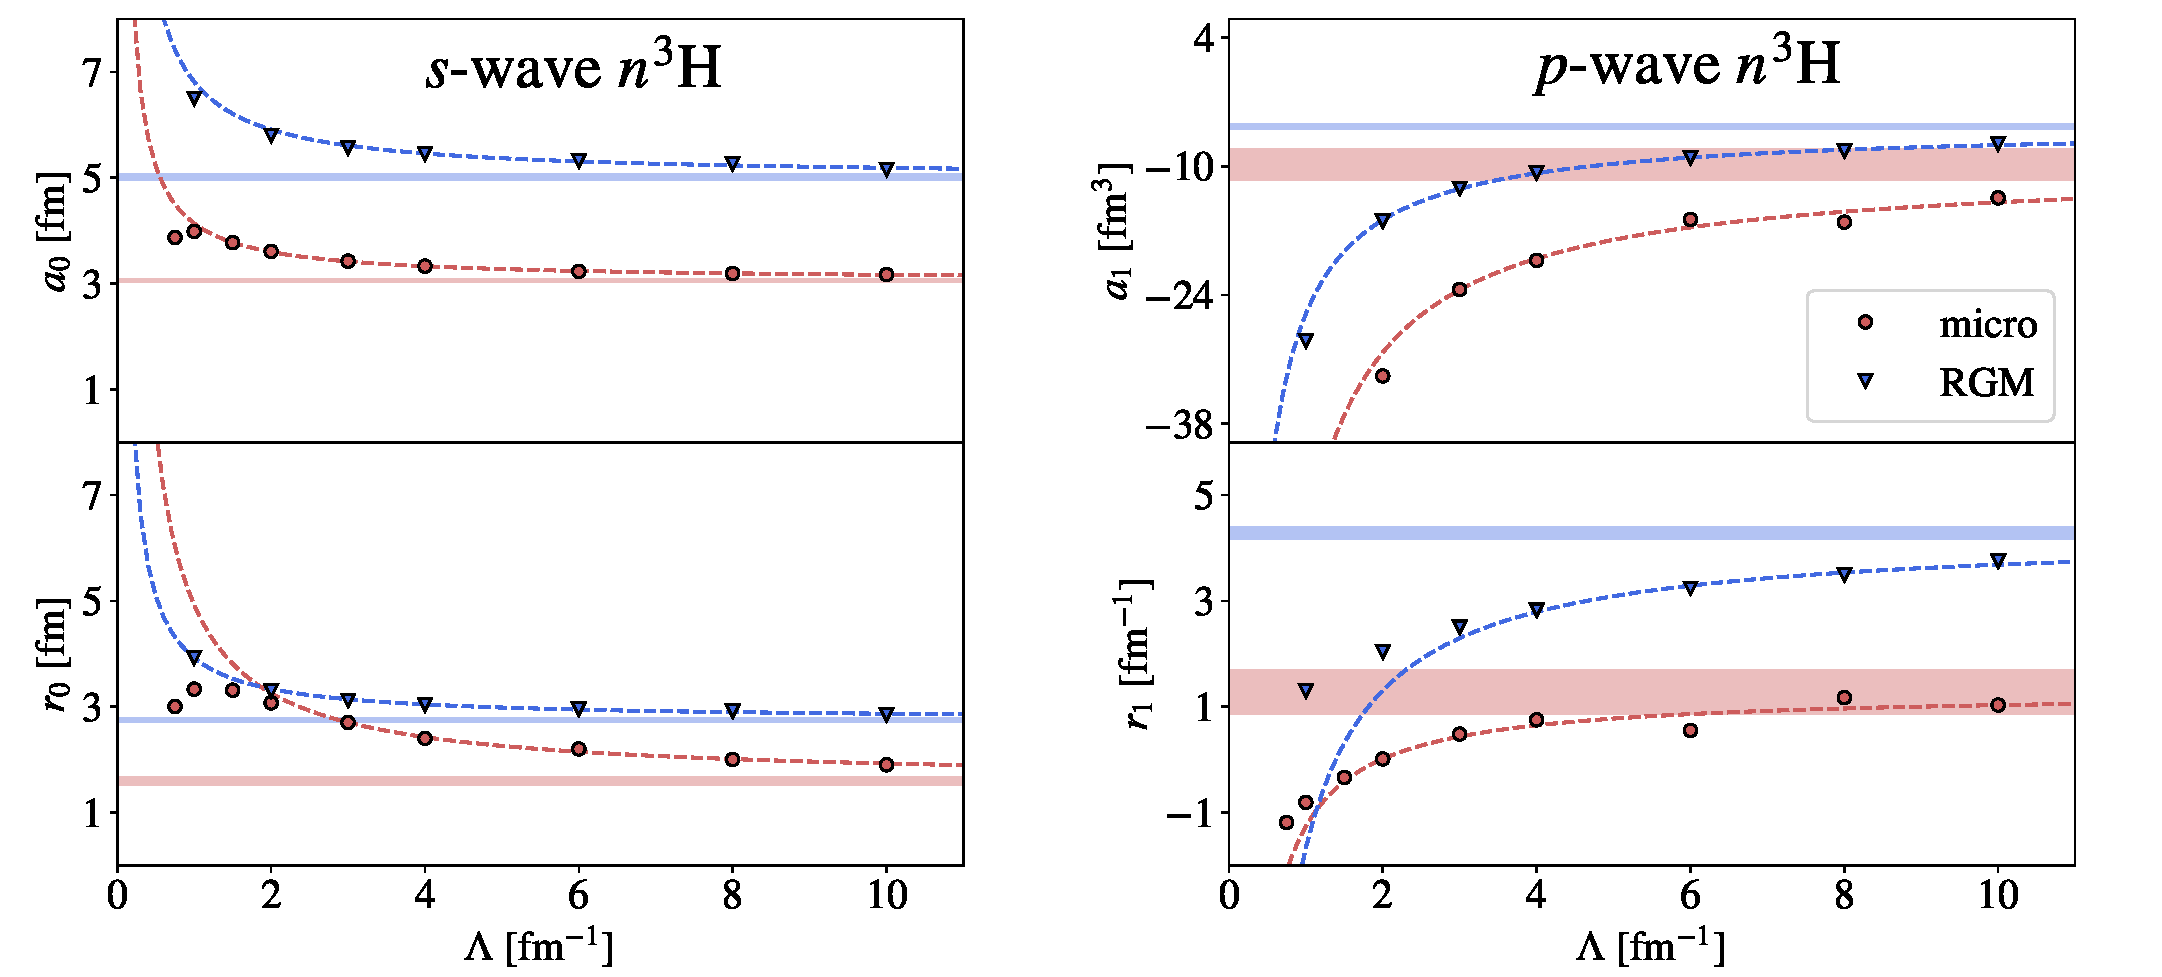
\includegraphics[width=\linewidth]{Graphs/ere.pdf}
  \caption{Cutoff and numerical-technique dependence of LO~\eftnopi~predictions
  for the leading two effective-range parameters (left panel: $S$-wave scattering length $a_0$ and effective range $r_0$;
   right panel: $P$-wave scattering volume $a_1$ and $r_1$)
   of the n-$^3$H scattering amplitude
  (SVM + Busch/Faddeev-Yakubovsky: red circle; 2-fragment RGM: blue triangle).
 The zero-range limit $\Lambda \rightarrow \infty$ (dashed lines) fits~\eqref{extrapolation}~to the discrete results
 (fit uncertainty: shaded bands).
 }
  \label{fig:ERE_Parameters}
\end{figure*}

%================================================
\subsection{Resonating Group Method}
%================================================
For neutron-projectile momenta much smaller than any excitation
scale of the triton, $k\ll k_{d-n}$, the description
of n-$^3$H scattering with a halo EFT~\cite{Hammer:2022lhx}~becomes appropriate. 
The resonating-group expansion
of the four-body wave function
resembles the accompanying transition from nuclear (``microscopic'') 
degrees of freedom to a fundamental trimer ($^3$H) and an atom (neutron)
field. Halo EFTs must account for exchange effects between particles within 
their elemental fields, \eg,
the Pauli repulsion between the projectile neutron and one of the neutrons 
inside the triton, via renormalization constraints, \ie,
through the introduction of, possibly redundant, (n-$^3$H)-interaction vertices.
The so-called resonating-group method can be employed such that its expansion of 
the wave function in a double
product of fragment-internal ($\phi$) and relative ($\chi$) states: 
\begin{equation}
\Psi=\sum_{a_j}\prod_{m=1}^{a_j}\phi^j_m\prod_{n=1}^{a_j-1}\chi^j_n\quad,
\end{equation}
and variations $\delta\Psi$ thereof, becomes formally identical to a cluster EFT. 
The compound fields of the halo EFTs
are identified with cluster states $\phi^j$ of a given partition $a_j$ of the $A$ 
nucleons, and the effective vertices
of the EFT are expressed in a set of integral kernels. Deriving the latter is 
tantamount to matching the halo EFT with
a microscopic, few-body description, and we achieve this matching analytically. 

In short, we utilize the technique with the same boundary conditions as in the FY 
approach~\eqref{eq:FYe_a} but find solutions
to the four-body Schr\"odinger equation in a subspace in which only variations 
of the relative function between the
triton-core $\psi_t$ and the neutron are admitted. Therefore 
(see~\cite{wildermuth1977unified}~for a pedagogical exposition),
the four-body problem reduces to a two-body for the relative 
motion between the triton and neutron.
With a Gaussian expansion of the core, the Gaussian regulated 
EFT potentials translate analytically into an effective
core-atom interaction with a local and a non-local, energy-dependent 
component which fully account for the identity and associated
permutation properties of the neutron projectile and its core copy:

\begin{equation}
\left(\hat{T}_{\rm rel}-E+\hat{U}^{(2)}_{\rm eff}(\ve{y})\right)\chi(\ve{y})+
\int\hat{U}^{(3)}_{\rm eff}(\ve{y},\ve{y}',E)\chi(\ve{y}')d\ve{y}'=0
\quad.\label{eq:rgm_sgl}
\end{equation}

No additional renormalization of the effective triton-neutron potentials 
is required, and we obtain their dependence
on $C_0$~\eqref{eq:vnn}~ and $D_0$~\eqref{eq:vnnn}~by analytically 
integrating out fast, \ie, core-internal degrees of freedom.
In effect,~\eqref{eq:rgm_sgl}~represents a halo EFT with two degrees of freedom: the extended but inert triton
and a neutron, with an interaction parametrized by the fundamental, nuclear theory.
A necessary matching constraint between the two descriptions is the wave function of the three-nucleon state, \ie, the core.
%This regulator dependent object is one source of numerical uncertainty.
To satisfy this constraint, we feed the single-particle 
densities of the SVM calculation
to the RGM integration over the fast degrees of freedom, thereby obtaining $\hat{U}^{(2/3)}_{\rm eff}$
as functions of the expansion coefficients of these densities in a set of
$\leq8$ Gaussian functions.

It remains to solve the integro-differential equation~\eqref{eq:rgm_sgl}, 
which is projected into partial waves, and we obtain the relative $S$- and $P$-wave functions
via a standard finite-difference method. The amplitude 
$a_L(k)$ is subsequently found with boundary conditions identical to~\eqref{eq:FYe_a},
albeit, for real momenta, only.
Although the numerical accuracy for the predictions of
ERE parameters and pole locations in this approach is inferior to the four-body formulations
due to the smaller breakdown momentum $k_{d-n}$, any divergence of an unrenormalized
amplitude or the convergence to zero, which the four-body problem might exhibit,
will be apparent in the RGM formulation.

%================================================
\section{Results and discussion}
%================================================

We shall first analyze the predictions of LO~\eftnopi for relative momenta in the n-$^3$H scattering system close to zero.
There, an ERE expansion of the amplitude is appropriate, and we extract its parameters with the microscopic methods 
(SVM + Busch Formula and FYE) as described above. 
For the scattering length $a_0$ and volume $a_1$,
we find relative agreement between two microscopic methods of order $\simeq 0.1-1 \%$ for $a_0$ and $\simeq 1-10\%$ for $a_1$ between the results. 
The effective ranges in $S$-wave ($r_0$) and $P$-wave ($r_1$) were extracted only via Bush formula and their numerical errors are not larger than $0.1$~fm and $0.1$~fm$^{-1}$, respectively.

The calculated $a_0,~r_0,~a_1$,~and~$r_1$ values using ab initio methods are shown as a function of increasing momentum cut-off $\Lambda$ in fig.~\ref{fig:ERE_Parameters}. 
As expected for \eftnopi LO observables, all scattering parameters converge as $1/\Lambda$. For $\Lambda \geq 4~{\rm fm^{-1}}$ we fit corresponding values using the function
\begin{equation}
    O(\Lambda) = O(\infty) +\frac{a}{\Lambda}
    \label{extrapolation}
\end{equation}
thus extrapolating calculated scattering parameters to the contact limit ($\Lambda \rightarrow \infty$). 
The resulting values extracted within \eftnopi at LO using the ``nuclear'' parametrization are: $a_0(\infty) = 3.06(1)$~fm, $r_0(\infty) = 1.59(7)$~fm for $S$-wave and $a_1(\infty) = -9.8(1.6)$~fm$^3$, $r_1(\infty) = 1.3(4)$~fm$^{-1}$ for $P$-wave, with extrapolation errors given in parentheses.
For the ``unitary'' $NN$ case we obtain $a_0(\infty) = 2.27(1)$~fm, $r_0(\infty) = 0.47(3)$~fm for $S$-wave n$^3$H scattering and $a_1(\infty) = -5.1(1)$~fm$^3$, $r_1(\infty) = 1.8(1)$~fm$^{-1}$ for $P$-wave n$^3$H scattering. 
%

%
In line with the sign convention adopted in eq. \ref{eq.app.ere}, the positive $a_0$ values suggest repulsive $S$-wave interaction, indicating dominance of Pauli principle between neutrons. 
This is in agreement with the lacking of bound state solutions in the $L=0^+$ n$^3$H channel for any $\Lambda$ considered. On the other hand, negative $a_1$s for all $\Lambda$ reveal attraction in $P$-wave n$^3$-H interaction. Approaching small-$\Lambda$ region, $|a_1|$ magnitude increases and the attraction becomes stronger, eventually resulting in the appearance of one $L=1^-$ bound state below $\Lambda\simeq$0.75 fm$^{-1}$. 
It is interesting to point out that, despite $S$-wave contact nature of the LO \eftnopi theory, the n$^3$H scattering has non-zero scattering volume and range components even in the $\Lambda \rightarrow \infty$ limit.
%

%
Comparing the ``unitary'' with the "nuclear" cases, both repulsion in $S$-wave and attraction in $P$-wave are preserved, however, for the former, the $a_0$ and $a_1$ are smaller in magnitude, which suggests in general weaker n-$^3$H interaction in the "unitary" case.
%
On a universal scale the scattering parameters can be expressed in
natural units of the three-body scale $R_3=1/\sqrt{-2mE_3/\hbar^2}\simeq 6$~fm: the only scale present in the system. 
In this case, the scattering parameters are reasonably natural and read $|a_0(\infty)|\simeq0.4\,R_3$, $|r_0(\infty)| \simeq 0.1\,R_3$, $|a_1(\infty)|^{1/3} \simeq 0.3\,R_3$, and $|r_1(\infty)|^{-1} \simeq 0.1\,R_3$. %** check the numbers, might be outdated **
%

\begin{figure*}
\centering
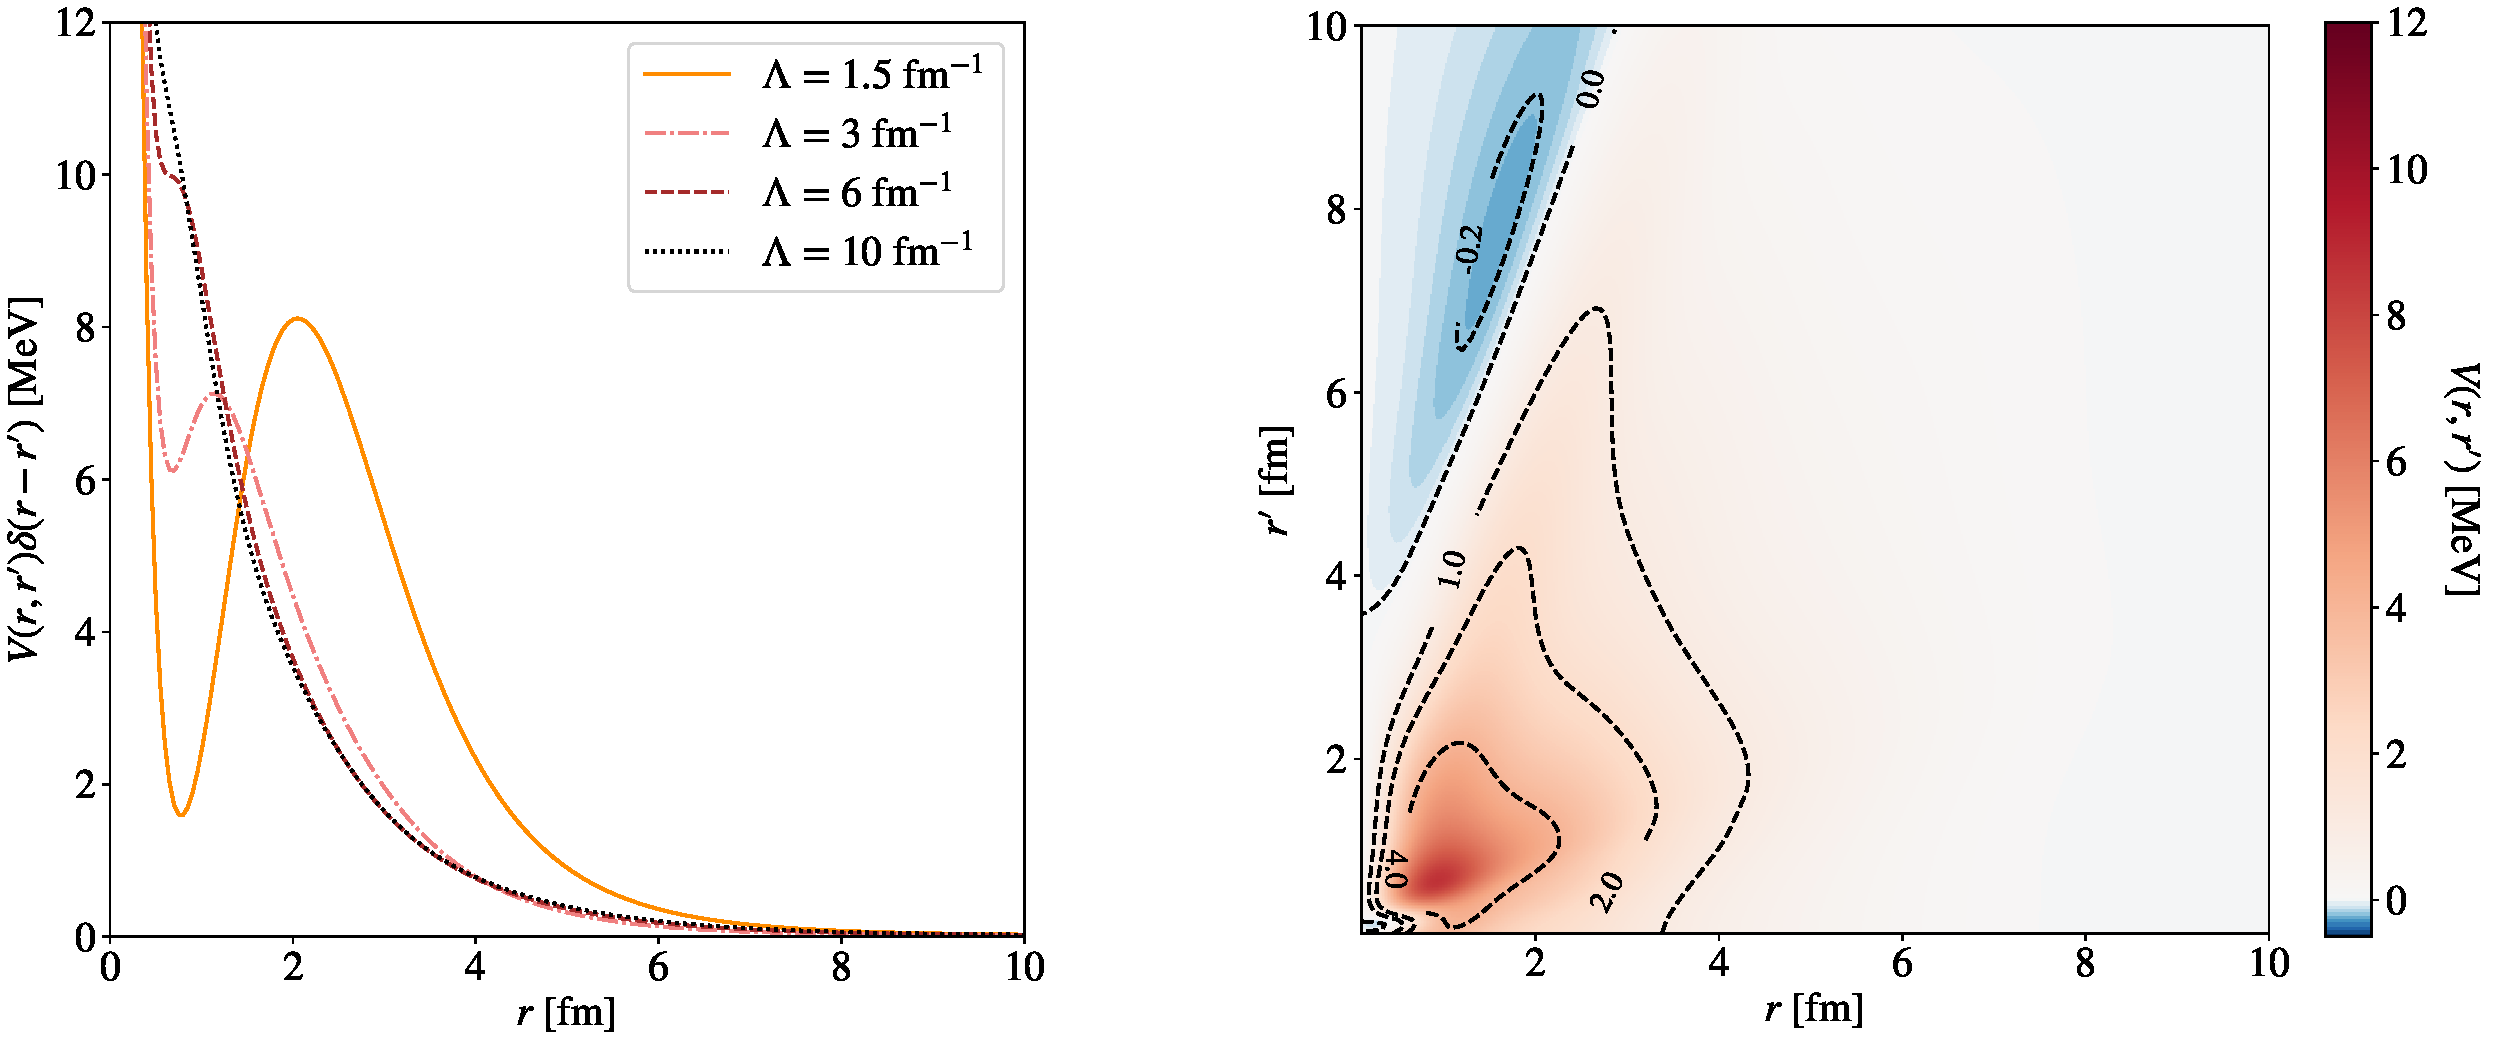
\includegraphics[width=\textwidth]{./Graphs/rgm}
%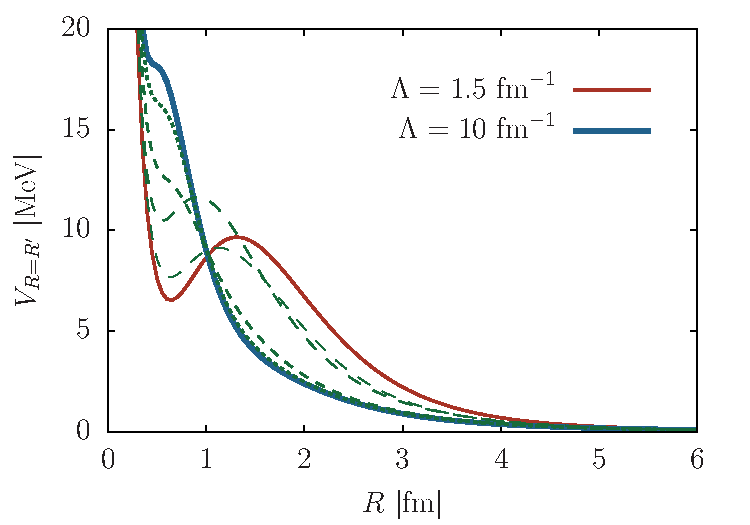
\includegraphics[width=.39\textwidth]{./Graphs/rgm_potential_unit}
%\hfill
%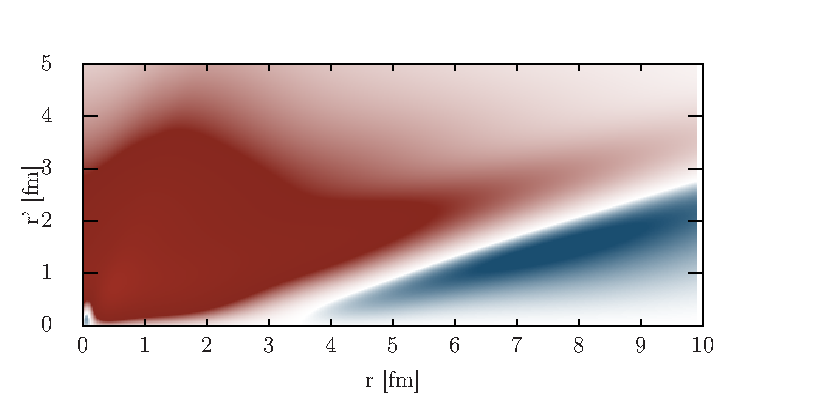
\includegraphics[width=.60\textwidth]{./Graphs/NonLocPot10_nuc}
\caption{Left panel: Local part of the effective $P$-wave n-$^3$H interaction $V(r,r')\delta(r'-r)$ as a function of the distance between the neutron and the center of mass of the triton. The interaction is extracted using the RGM at the n-$^3$H zero energy and evaluated for different cut-offs from 1.5 (red line) to 10~fm$^{-1}$ (blue line); intermediate cut-offs are shown as green dashed lines. Right panel: Same as in the left panel but full non-local $V(r,r')$ interaction calculated for cutoff $\Lambda=10$~fm$^{-1}$.}\label{Fig:Potential}
\end{figure*}

%
A comparison with the experimental data and the other theoretical models can only be done in $S$-wave (no data are available for scattering volumes and ranges). However, the $a_0$ calculated with ab initio methods as well as the RGM result appears to be compatible in sign and magnitude with the realistic calculations and experimental results available (inside \eftnopi truncation error), for both the ``nuclear'' and ``unitary'' parametrization used. 
As reference for theory and experiment we use the average scattering parameters $a_0^c=\sqrt{0.25(3a_{(S=1)}^2+1a_{(S=0)}^2)}$:   $a_0^{theo}=3.71$ fm\cite{Lazauskas:2019hil} and $a_0^{exp}=2.9\,-\,4.3$ fm\cite{Tilley:1992zz}, 
which are in good agreement with \eftnopi prediction considering the LO truncation uncertainty. 
%

%
Using the RGM method, the scattering parameters found are
$a_0(\infty) = 5.71$~fm, $r_0(\infty) \simeq 0.$~fm, $a_1(\infty) = -10.49$~fm$^3$, and $r_1(\infty) = 4.33$~fm$^{-1}$ for the ``nuclear'' parametrization; and
$a_0(\infty) = 3.3$~fm, $r_0(\infty) \simeq 1.8$~fm, $a_1(\infty) = -2.5$~fm$^3$, and $r_1(\infty) = 10.1$~fm$^{-1}$ fo the ``unitary'' case. 
These results are relatively distant from the ab initio calculation, however, it is hard to estimate the error introduced by the approximations done in the method and how they correlate with the expansion parameter of the theory.
Moreover, the RGM results appear to be highly sensitive to the $^3$H wave function used in the calculation, introducing a further dependence of the results from the input choice.
The result of RGM appear also to be natural and convergent (see Fig. \ref{fig:ERE_Parameters}) in the large cut-off limit.
%maybe we can add few more comments on this, but nothing comes in my mind.

%

%



%

%
\vspace{2mm}
%
Although the effective n-$^3$H interaction is not an observable, we use the RGM to extract its $P$-wave
component to acquire a deeper insight into interplay between repulsive and attractive parts and their evolution with $\Lambda$. In fig.~\ref{Fig:Potential}, we visualise such interaction for the "nuclear" case and zero-energy scattering.
%

%
On the left panel, the local part of the coordinate space interaction ($r=r'$) is shown as a function of the distance between the neutron and the center of mass of the triton. 
A positive energy pocket at distance $r\simeq0.5$~fm can be noticed for small cut-offs, however, it vanishes approaching the contact limit ($\Lambda\to\infty$). 
Remarkably, with only the local part of interaction, no resonance can emerge.
%

%
On the right panel, the full coordinate interaction $V_{n-t}(r,r')$ is plotted for $\Lambda=10$~fm$^{-1}$ and zero energy.
The non-symmetry of the interaction is a consequence of the folding technique. 
Here, the repulsive part of the interaction (red) clearly dominates and it can be traced as a combination between the repulsion induced by three-body forces, two-body exchange interaction, and centrifugal barrier. 
One can notice a weak attraction pocket ($min(V_{n-t})\approx$-0.35 MeV; blue) present far from the diagonal. 
The minimum of this pocket is too small to support a bound state, but it might be the reason for the appearance of a broad resonance state. This pocket is retained even for larger cut-offs. 

\begin{figure*}
\centering
  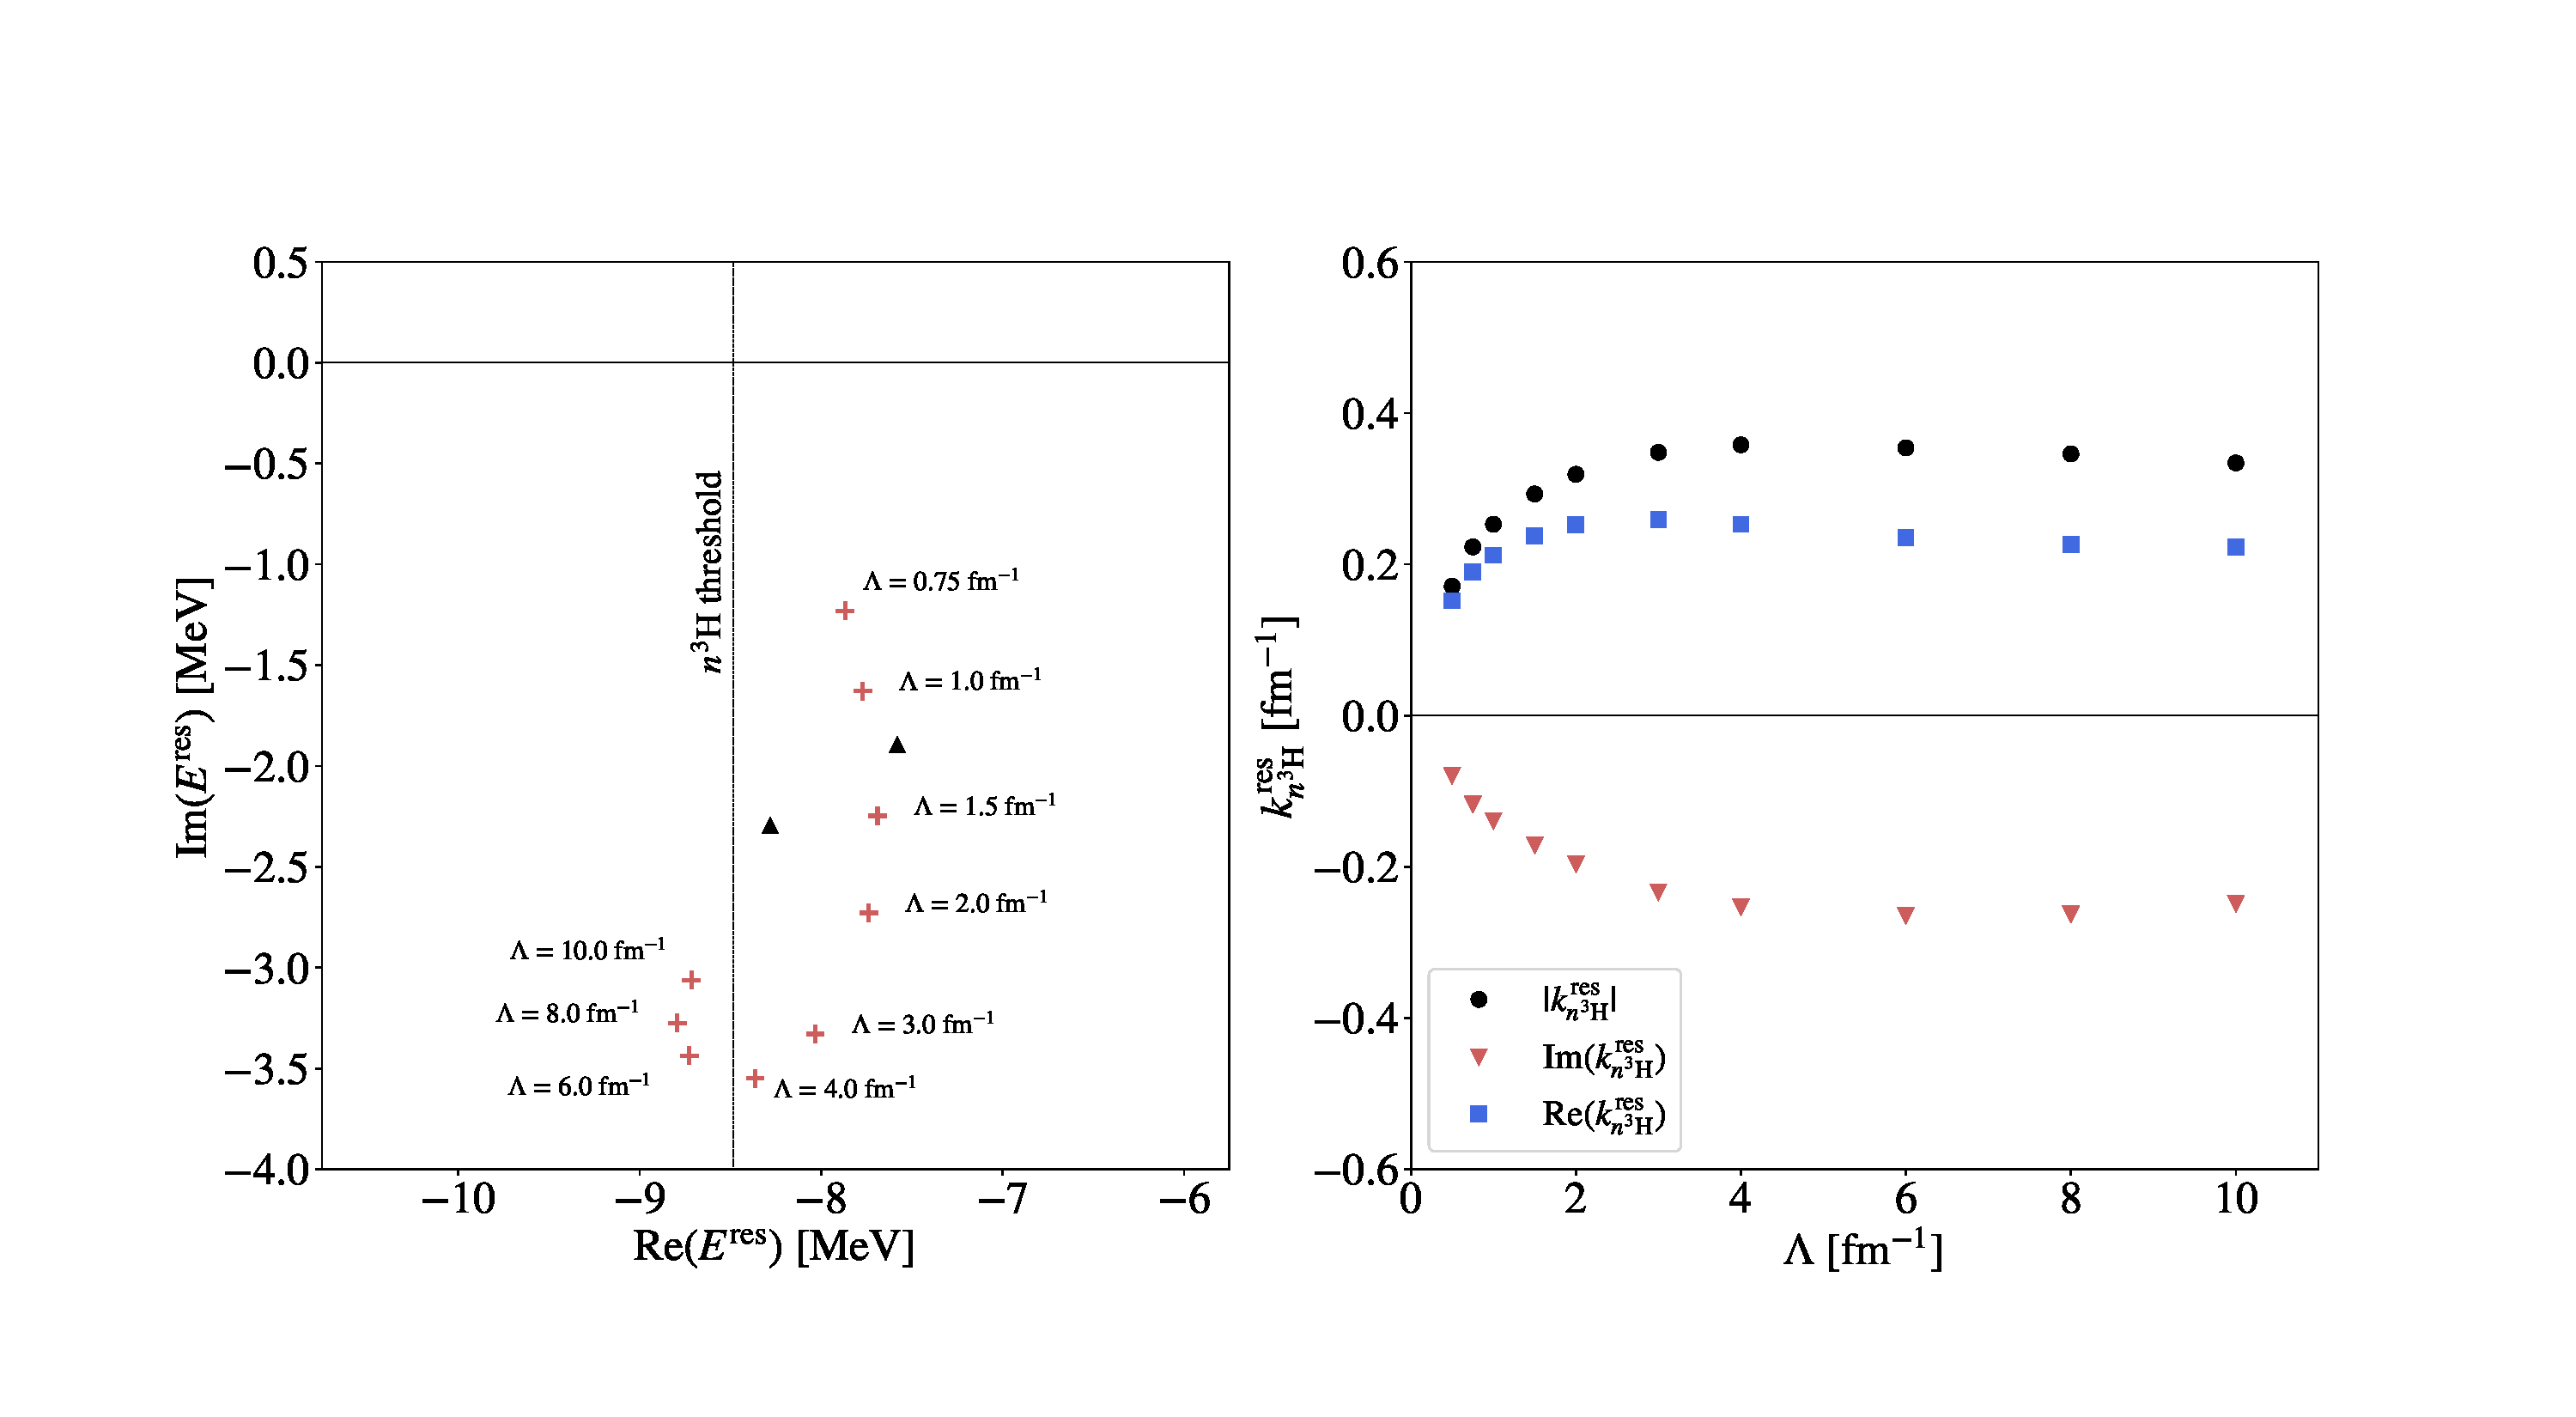
\includegraphics[width=.98\linewidth]{Graphs/resonance.pdf}
  \caption{ Left panel : Complex energy plane with calculated $^4$H $1^-$ resonance positions (red crosses) for multiple momentum cutoff $\Lambda$. 
  The black triangles represent the position of the $1^-$ resonance extracted in Ref~\cite{Lazauskas:2019cxj}
  Right panel: The absolute value, real, and imaginary part of the complex resonance momentum $k^{res}_{n ^3{\rm H}}$ as a function of increasing $\Lambda$. The momentum is related to resonance energies via eqs.~\ref{mmnt}~and~\ref{kreim}. The resonance pole was extracted directly solving the four-nucleon problem trough the Faddeev-Yakubovsky equations.}
  \label{fig:Pole_PositionN}
\end{figure*}

%
So far our calculations revealed non-vanishing $P$-wave attraction in n-$^3$H scattering in the contact limit, suggested by the negative $a_1(\infty)$, and the existence of attractive pocket in the effective n$^3$H $P$-wave RGM potential which persists even at highest considered cut-off $\Lambda=10$~fm$^{-1}$. Both of these results lead us, yet still not quite firmly, to an existence of a broad $^4$H resonance stabilizing with increasing momentum cut-off. 
%

%
The final step in our calculation is to search directly for a position of the $J^\pi=1^-$ nuclear resonance looking for a pole of a 4-body S-matrix. This has been done by solving the Faddeev-Yakubovsky equations.
Results are are displayed in fig.~\ref{fig:Pole_PositionN}.
In the left panel, the pole trajectory as function of the cutoff, using the ``nuclear'' interaction, is shown in the complex energy plane. 
It can be followed to pass the n$^3$H threshold energy $B_{t}=8.484$~MeV (denoted by dashed vertical line) finally stabilizing around $E^{res}=-8.7-i\,3.1$ for cutoffs greater than $6$~fm$^{-1}$. The passage of the resonance position from the fourth quadrant (${\rm Re}(E)>0$; ${\rm Im}(E)<0$) into the subthreshold third quadrant (${\rm Re}(E)<0$; ${\rm Im}(E)<0$) makes difficult to clearly visualise the convergence of the the resonance position with increasing $\Lambda$. 
Therefore, we transform calculated resonance energies into n-$^3$H complex momenta $k^{res}_{n ^3{\rm H}}$  
\begin{equation}
    k^{res}_{n ^3{\rm H}} = \sqrt{2 \mu E^{res}_{n ^3{\rm H}}},~~~~E^{res}_{n ^3{\rm H}}= E^{res} + B_{t},
    \label{mmnt}
\end{equation}
where $\mu \approx 3/4 m$ is the reduce mass of the two-body n-$^3$H system. The real and imaginary part of the complex momentum then can be evaluated as  
\begin{equation}
    \begin{split}
        {\rm Re}(k^{res}_{n ^3{\rm H}}) &= \sqrt{\frac{2\mu \left(|E^{res}_{n ^3{\rm H}}|+{\rm Re}(E^{res}_{n ^3{\rm H}})\right)}{2}},\\
        {\rm Im}(k^{res}_{n ^3{\rm H}}) &=  {\rm sgn}\left({\rm Im}(E^{res}_{n ^3{\rm H}})\right)\sqrt{\frac{2\mu \left(|E^{res}_{n ^3{\rm H}}|-{\rm Re}(E^{res}_{n ^3{\rm H}})\right)}{2}}.\\
    \end{split}
    \label{kreim}
\end{equation}

The ${\rm Re}(k^{res}_{n ^3{\rm H}})$, ${\rm Im}(k^{res}_{n ^3{\rm H}})$, and $|k^{res}_{n ^3{\rm H}}|$ momenta are plotted as a function of $\Lambda$ in the right panel of fig.~\ref{fig:Pole_PositionN}.  
For cut-off values larger than the breakup scale of the theory $m_\pi$ the resonance momentum starts to stabilize and its absolute value $|k^{res}_{n ^3{\rm H}}|$ does not exceed $0.35~{\rm fm}^{-1}\simeq 0.5 m_\pi$, remaining well inside the convergence radius of the theory (I.e., we do not expect subleading contributions to be able to remove this state from the theory).
%

%
We notice that the resonance position can also be found as pole of the n-$^3$H T-matrix in eq. \ref{eq:Tmatrix} parametrized by the scattering parameters calculated using \eftnopi. 
Truncating the ERE at the scattering volume we expect a deviation from the \eftnopi resonant momentum of $\Gamma_{halo}$: the expansion parameter of the n-$^3$H halo EFT at the resonant energy.
Doing this exercise we find a resonant momentum of $k^{res}_{halo})\simeq80+46\,i$ MeV, which is compatible, in the truncation error of the halo EFT, with the momentum of the \eftnopi pole ($k^{res}_{n ^3{\rm H}}\simeq46+49\,i$MeV).
Confirming that the pole is also inside the convergence value and can be treated in halo EFT.  
%

%
Comparing our $^4$H resonance result with experimental data and previous calculations, the major difference is that our pole goes to the subthreshold region in the $\Lambda\rightarrow\infty$ limit, namely, the resonance energy is lower than the n$^3{\rm H}$ threshold energy. 
Notice, however, that this kind of states are not bound despite their negative energy, and remain non normalizable.
Theoretically, this is not an issue since the pole existence in subthreshold region does not break causality and it can be moved in the standard resonant region by a continuous transformation of the interaction (e.g. reversing the renormalization group transformation) and, possibly, by the inclusion of \eftnopi subleading orders. 
% I dont like this statement bc the LO is compatible with a normal resonance and we expect this pole to go in the correct physical position at a certain point in the pionless expansion
%However, such a subthreshold resonance has only small impact on the physical observables and thus its signature would be almost impossible to be detected in an experiment.
%

%
Due to the difficulty of comparing different experimental set-up and theoretical calculations, it is hard to state to which extent our $^4$H resonance calculation is in agreement with the others in quantitative terms. 
%
To stress this point, one can notice that the S-matrix pole real part of the energy is, in general, smaller than the one extracted with R-matrix analysis.
An illustrative example is provided by the  transfer reactions $^2$H(t,p)$^4$H and $^3$H(t,d)$^4$H \cite{Sidorchuk:2004ntw}. 
The R-matrix analysis of the results obtains for the lowest $^4$H state $E_R$=3.05$\pm$0.19 MeV and $\Gamma$=4.18$\pm$1.02 MeV while the corresponding S-matrix pole, extracted by the same authors, led to $E_R$ =1.99$\pm$0.37 MeV and $\Gamma_R$=2.85$\pm$0.3 MeV. 
Therefore, a fair comparison can only be done with other S-matrix pole predicted with realistic interactions. 
%
The study done in refs~\cite{Lazauskas:2019hil,Arai:2003ek, deDiego:2007rd} found a pole corresponding to ${\rm Re}(E_r)=(0.9\,-\,1.23)$~MeV and $\Gamma=(3.5\,-\,5.8)$~MeV.
\eftnopi at LO predicts a slightly less energetic but much narrower resonance ($E_r=-0.22$~MeV and $\Gamma=1.6$~MeV). 
The maximum relative distance between the poles momentum is $\sim 80\%$ of the total energy, although a large difference, it is in line with the expected uncertainty of the powercounting truncation.
%

%
The same calculations have been repeated using the ``unitary'' $NN$ interaction. In this case, Faddeev-Yakubovsky calculations find a wider resonance than in the nuclear case at energy $E_r=-8.156$~MeV and $\Gamma=2.4$~MeV (equivalent to absolute momentum $k_{n-t}=0.58\,m_\pi$). 
Despite this pole being relatively close to the one previously calculated (40\% of relative error: in line with the SU(4) assumption expected uncertainty), it is extremely hard to be tracked and has been studied only for cut-offs compatible with $m_\pi$: $\Lambda=0.75$ and $2$ fm$^{-1}$, and was not possible to check its value in the contact limit.


%================================================
\section{Conclusions}
%================================================
%
In this work, we observe the existence of a stable $J^{\pi}=1^-$resonance in $^4$H using the pionless effective field theory (\eftnopi) truncated at leading order. The calculation is done using microscopic ab initio techniques as well as employing a folded interaction using the resonating group method (RGM).
%
Although other works have already established the possibility of creating shallow resonances using \eftnopi in $S$-wave two-nucleons and hypernuclear systems, this is the first time a stable $P$-wave
resonance has been found within this framework. 
%The scattering observables we calculate appear to be natural when compared with the fixed three body scale.
%
To supplement our ab initio calculation, we repeated it using the RGM, fixing as calculation input the $^3$H wavefunction using the density calculated with ab initio method.
The result found for the scattering parameter are qualitatively similar, but deviate from the results calculated using ab initio methods.
However, the uncertainty of the method is hard to be estimated a priori, both for the assumption of having a frozen core $^3$H and for the sensibility to the input wave function.
Nonetheless, the RGM results appear to be cut-off convergent and natural in the contact limit.
%

%
The values of the resonance energy and of the scattering parameters extracted from S-matrix formalism and from experiment can be hardly compared because of the very different way of extracting them, the different interpretation of the resonant state, and the difference among the experimental setups and protocol. 
However one can compare the S-matrix resonant poles among different theoretical calculations. \eftnopi find a resonance that is sharper than other calculations performed with realistic interactions. However, the calculations are still in agreement considering the \eftnopi LO truncation uncertainty. Comparing the result of different parametrizations of the EFT LO, namely starting from a two-body interaction that reproduces the deuterium binding energy or from a unitary interaction, we find a difference that is again in agreement with the expected uncertainty given by assuming a spin-independent interaction.
%
On the qualitative point of view, the major difference between \eftnopi and the resonances found in literature is the subthreshold nature of the former in the contact limit. 
However, this is not fundamentally a problem, in part because these pole can be physical\cite{formartinanyexample}, and because a non-subthreshold resonance may still be obtained introducing higher orders of the EFT expansion.
%

%
The possibility of creating $P$-wave many-body poles using a contact $S$-wave theory is remarkable. 
Moreover, it also has strong implications for \eftnopi powercounting, possibly solving the issue of the absence of stable bound states states for nuclei larger than $^4$He at LO. 
We conjecture that an existing $P$-wave resonance might be moved on the stable region by the insertion of sub-leading orders.
This would be trivially impossible if no $P$-wave states are present at all.

\section*{acknowledgement}
We thank H.~W.~Grie\ss hammer, N.~Walet, and U.~van Kolck for helpful discussions. 
MS was supported by the Pazy Foundation and the Israel Science Foundation grant 1086/21,
JK by the US Department of Energy under contract DE-SC0015393, and
LC and JC in part by the National Science Foundation under Grant No. NSF PHY-1748958.



\bibliographystyle{ieeetr}

%elsarticle-harv}
\bibliography{bibi.bib}

\end{document}